%%%% This Beamer example was created by LianTze Lim, April 2017.

%%%% This is a VERY simple and minimalistic beamer theme,
%%%% even reminiscent of marker pens on transparencies!
%%%% It mimics the look of the "seminar" package, which
%%%% can only be used with plain TeX.
%%%% There are also some comments and example to show how
%%%% to customise various elements, e.g. the font and colours.

\documentclass[12pt, usenames, dvipsnames]{beamer}
%% If you'd like the default font size to be even larger, use 14pt or 17pt; these are supported by Beamer.

\usepackage[english]{babel}
\usefonttheme{professionalfonts} % using non standard fonts for beamer
\usefonttheme{serif}
\usepackage[utf8]{inputenc}
\usepackage[T1]{fontenc}
\usepackage{lmodern}
\usepackage[absolute,overlay]{textpos}
\usepackage{physics}
\usepackage{amsmath}

%%%%%%%%%%%%%%%%%%%%%%%%%%%%%%%%%%%%%%%%%
% These lines should usually go into a .sty file,
% but I'll leave them here so that it's easier to
% see how to customise a Beamer theme.
% Remember, the Beamer manual is your friend!!
% http://texdoc.net/pkg/beamer
%
%% So if your re-definitions have a @ somewhere, you
%% _MUST_ put a \makeatletter before these lines and then
%% \makeatother after them. This trick can only be done
%% in the preamble! BUT if you're doing these re-definitions
%% in a .sty file (so that you \usepackage it later), you
%% don't need the \makeatletter and \makeatother.
\makeatletter

%% Set the left and right margins
\setbeamersize{text margin left=1em,text margin right=1em}

%% FONTS
\setbeamerfont{title}{series=\bfseries,size=\LARGE}
\setbeamerfont{subtitle}{series=\bfseries,size=\Large}
\setbeamerfont{frametitle}{series=\bfseries,size=\small}
\setbeamerfont{block title}{series=\bfseries,size=\normalsize}
\setbeamerfont{footline}{size=\normalsize}

%% COLOURS
%% If you'd like everything to have the same colour
\usebeamercolor{structure}
\setbeamercolor{normal text}{fg=structure.fg}
\usecolortheme[named=Black]{structure}

%% Add a line after the frametitle
\addtobeamertemplate{frametitle}{}{\vspace*{-1ex}\rule{\textwidth}{1pt}}

%% Use circular discs as itemized list markers;
%% there's an existing option in Beamer for it so I'll use it
\setbeamertemplate{itemize items}[circle]
\setbeamertemplate{bibliography item}{\insertbiblabel}

%% Remove default navigation symbols (We'll add the ones we need in the footline
\setbeamertemplate{navigation symbols}{}


%% And before the footline... actually we'd like to re-define
%% the footline
\setbeamertemplate{footline}{%
   %% Beamer headlines and footlines are always full-paperwidth, so if you want the horizontal line to
   %% not span it entirely you'll need to do a bit of arithmetic
   \centering
   \begin{minipage}{\dimexpr\paperwidth-\beamer@leftmargin-\beamer@rightmargin\relax}
   \centering
   \rule{\linewidth}{1pt}\vskip2pt
   \usebeamerfont{footline}%
   \usebeamercolor{footline}%
   %% The frame number smack in the middle
   \hfill\insertpagenumber/\inserttotalframenumber
   \hfill%
   %% ONLY the navigation symbols we want at the far right.
   %% We use an \llap so that it takes up zero width, and doesn't throw the page number off-centre!
   \llap{\insertframenavigationsymbol\insertbackfindforwardnavigationsymbol}\par
   \end{minipage}\vskip2pt
}

\makeatother
%%%% END STYLE CUSTOMISATION %%%%%%%%%%%%



\title{Momentum Distribution Properties of Ultracold Particles}
\author{Tim Skaras, Shah Saad Alam, Li Yang, Han Pu}
\institute{\small Rice University}
\date{15 October 2018}

\begin{document}

%% Slide 1

\begin{frame}
  \titlepage

\end{frame}

% Uncomment these lines for an automatically generated outline.
%\begin{frame}{Outline}
%  \tableofcontents
%\end{frame}

\section{Introduction}

%% Slide 2

\begin{frame}[t]{Introduction}

\begin{block}{Research Summary}
\begin{itemize}
	\item We study strongly-interacting, ultracold particles confined in a one-dimensional harmonic trap
	\item Strongly-interacting 1D systems often exhibit peculiar quantum behavior
\end{itemize}
\end{block}

\begin{block}{Two Central Questions:}
\begin{itemize}
	\item How does the momentum distribution decay for large momentum (e.g., exponentially, inverse power law)?
	\item What happens to momentum distribution when trapping potential is turned off?
\end{itemize}
\end{block}

\end{frame}

%% Slide 3

\begin{frame}[t]{Introduction}

\begin{block}{Relevant Factors}

\begin{itemize}
	\item Particle type (e.g., fermion, boson, anyon)
	\item Particles with spin degree of freedom
	\item Systems with non-zero temperature
	\item Number of particles
	\item Interaction strength
\end{itemize}

\end{block}

\end{frame}

\section{Background}

\subsection{Types of Particles}

%% Slide 4

\begin{frame}[t]{Background: Types of Particles}

\begin{block}{Bosons and Fermions}
\begin{itemize}
\item In nature, we only observe bosons and fermions
\item Distinguishing characteristic is how their wavefunctions behave when two particles are exchanged
\end{itemize}

\[ \psi_{B}(x_{1}, x_{2}) =  \psi_{B}(x_{2}, x_{1}) \]
\[ \psi_{F}(x_{1}, x_{2}) =  -\psi_{F}(x_{2}, x_{1}) \]

\begin{itemize}
\item Exchange Statistics: how wave function behaves under particle exchange
\item Identical particles $\rightarrow$ exchanging particles can only change $\psi$ by complex phase
\end{itemize}

\end{block}

% Commands to include a figure:
%\begin{figure}
%\includegraphics[width=\textwidth]{your-figure's-file-name}
%\caption{\label{fig:your-figure}Caption goes here.}
%\end{figure}

%% Add slide to talk about Pauli Exclusion Principle

\end{frame}


%% Slide 5

\begin{frame}[t]{Background: Types of Particles}

% Explain what an anyon is and mention applications

\begin{block}{Anyons}

\begin{itemize}
\item As a theoretical idea, we can define another type of particle -- the anyon
\item Described by its anyonic statistic $\kappa \in [0,2)$ 
\item Defining characteristic:
\[ \psi_{\kappa}(x_{1}, x_{2}) = e^{i \pi \kappa \epsilon(x_1 - x_2)} \psi_{\kappa}(x_{2}, x_{1})  \]

% Include verbal explanation of epsilon sign function
where $\epsilon(x)$ is the sign function

\item $\kappa  = 0 \rightarrow e^{i \pi \kappa} = 1 \rightarrow$ Bosons
\item $\kappa  = 1 \rightarrow e^{i \pi \kappa} = -1 \rightarrow$ Fermions
\end{itemize}
\end{block}

% Insert line graph from poster relating kappa to bosons and fermions

\end{frame}

\subsection{Strong Interaction}

%% Slide 6

\begin{frame}[t]{Background: Strong Interaction}

% Explain what hard core is and give hamiltonian
\begin{block}{Hard-Core Particles}
\begin{itemize}
\item We consider systems `hard-core' particles: infinite, repulsive contact interactions
\item Means that no two of the particles can occupy same position
\item If particles are spinless, we can write the Hamiltonian
\[ H = \sum_{j = 1}^{N} \left[ \frac{-1}{2} \pdv[2]{}{x_{j}} + \frac{1}{2}x_j^2 \right]
	+ g \sum_{j < \ell} \delta(x_j - x_\ell) \]
where $\hbar = m = \omega = 1$ and in the hard-core limit $g \rightarrow \infty$

\item Our research will consider hard-core bosons and hard-core anyons
\end{itemize}


\end{block}

% For most part, we study hard-core bosons or hard-core anyons

\end{frame}

\section{Methods}

%% Slide 7

\begin{frame}[t]{Methods: Mappings}

% How do we calculate the momentum distribution for hard-core bosons or anyons?
\begin{block}{Bose-Fermi Mapping}
\begin{itemize}
\item Bosons and fermions are very different, but hard-core bosons (HCB) are similar to fermions (e.g., no two can occupy same position)
\item M. Girardeau (1960) showed there was a mapping between these two systems
\item Procedure for turning $N$-particle fermion solution into boson solution
\[ \psi_{B}(x_1,\ldots, x_N) = A(x_1,\ldots, x_n)\psi_F(x_1,\ldots, x_N) \]
\[ A(x_1,,\ldots, x_N) = \prod_{1 \leq \ell < j \leq N}  \epsilon(x_j - x_\ell) \]
\end{itemize}
\end{block}

% Explain importance and use of Bose-Fermi Mapping as well as Anyon-Fermion Mapping

\end{frame}

%% Slide 8

\begin{frame}[t]{Methods: Mappings}

% How do we calculate the momentum distribution for hard-core bosons or anyons?
\begin{block}{Anyon-Fermion Mapping}
\begin{itemize}
\item Girardeau (2006) showed mapping existed for hard-core anyons (HCA)
\item Procedure for turning fermionic solution into bosonic solution
\[ \psi_{\kappa}(x_1,\ldots, x_N) = A_\kappa(x_1,\ldots, x_N)\psi_F(x_1,\ldots, x_N) \]
\[ A_{\kappa}(x_1,\ldots, x_N) = \exp(i \pi (1 - \kappa) \sum_{1 \leq \ell < j \leq N} \theta(x_j - x_\ell)) \]
where $\theta$ is the heaviside theta function
\end{itemize}
\end{block}

% Explain importance and use of Bose-Fermi Mapping as well as Anyon-Fermion Mapping

\end{frame}

%% Slide 9

\begin{frame}[t]{Methods: One Body Density Matrix}

% Give expression for the OBDM and the momentum distribution
\begin{itemize}
\item After obtaining the wave function for our system using the mappings, we study its properties using the One-Body Density Matrix (OBDM)

\[ \rho(x, x') = \int_{-\infty}^{\infty} dx_2 \cdots dx_N \psi^*(x,x_2,\ldots, x_N) \psi(x',x_2,\ldots, x_N) \]

\item Then, we use this to find an expression for the momentum space density profiles
\[ n(p) = \frac{N}{2\pi} \int_{-\infty}^{\infty} dx \int_{-\infty}^{\infty} dx'
		e^{ip(x-x')} \rho(x,x')  \]
\item Difficult to solve analytically, even for two hard-core bosons

\end{itemize}

\end{frame}

%% Slide 10

\begin{frame}[t]{Methods: Momentum Space Density Profiles}

%[Include plot of $n(p)$ for hard-core bosons, fermions, and hard-core anyons to help people visualize]

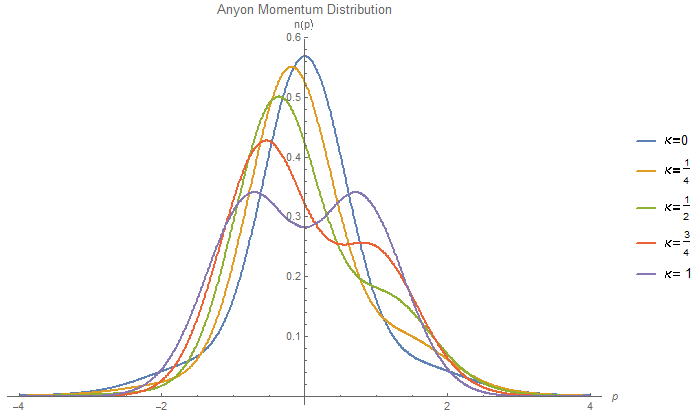
\includegraphics[width=\textwidth]{AnyonMomentums}

% Show plot of n(p) for HCB or HCA or something to help them visualize

\end{frame}


%% Slide 11

\begin{frame}[t]{Background: Two Hard-Core Bosons}

% Describe process to find Tan Contact

\begin{block}{Tan Contact}
\begin{itemize}
\item Momentum distribution for spinless fermions in a harmonic trap will decay exponentially
\item Minguzzi et al. (2002) showed for 2 spinless hard-core bosons
\[ \lim_{p \rightarrow \infty} n_{B}(p) = \frac{C_{B}}{p^4} = \left( \frac{2}{\pi} \right)^{3/2} \frac{1}{p^4} \]
where $C_B$ is the Tan Contact (see Tan (2008)) or momentum tail coefficient
\end{itemize}
\end{block}

% Include relevant plots

\end{frame}

%% Slide 12

\begin{frame}[t]{Background: Two Hard-Core Bosons}
\begin{block}{Dynamical Fermionization}
\begin{itemize}
\item Hard-core bosons and fermions have different momentum distributions
\item When trapping potential is turned off for hard-core bosons, Minguzzi et al. (2005) showed that 
\[ \lim_{t \rightarrow \infty} n_{B}(p; t) = n_{F}(p) \]
using a scaling transformation
\item This process is known as dynamical fermionization

\end{itemize}
\end{block}
\end{frame}

\section{Progress}

%% Slide 13

\begin{frame}[t]{Progress: Two Hard-Core Anyons}

% Describe process to find Tan Contact

\begin{block}{Tan Contact}
\begin{itemize}
\item Calculate Tan Contact for two hard-core anyons
\[ \lim_{p \rightarrow \infty} n_{\kappa}(p) = \frac{C_{\kappa}}{p^4} =  \cos^2 \left(\frac{\pi \kappa}{2} \right) \frac{C_{B}}{p^4} \]
\item And numerically showed dynamical fermionization occurs
\end{itemize}


\end{block}

\end{frame}

% Slide 14

\begin{frame}

\begin{center}
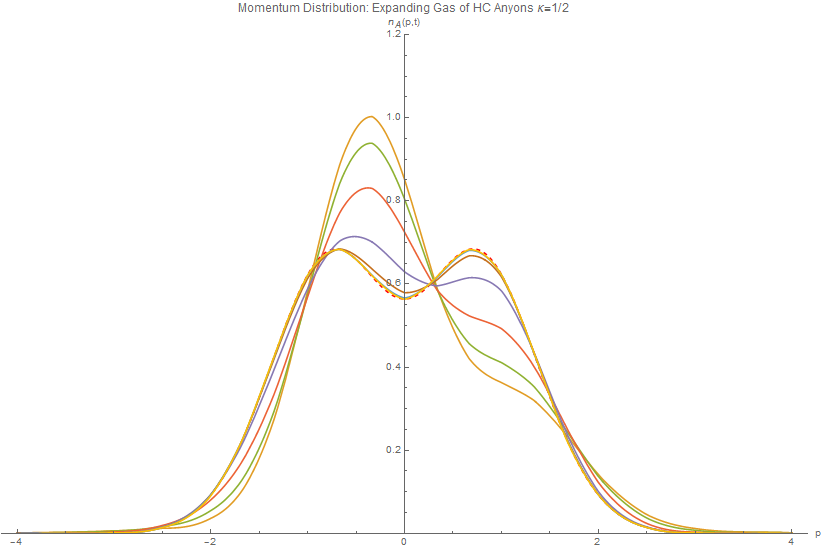
\includegraphics[width=\textwidth]{MomDistExpandingAG}
\end{center}

\end{frame}

%% Slide 15

\begin{frame}[t]{Progress: Finite Temperature Tan Contact}
\begin{itemize}
\item Hao et al. (2017) calculate the Tan Contact for N Hard-core Anyons at finite temperature in grand canonical ensemble

\item Their calculation more or less follows Vignolo et al. (2013)

\begin{multline*}
\rho_{B}(x, y) = \sum_{N, \alpha} P_{N, \alpha} N \int_{-\infty}^{\infty} dx_2 \cdots dx_N \psi_{N, \alpha}(x, x_{2}, \ldots, x_N) \\ \times  \psi^*_{N, \alpha}(y, x_2, \ldots, x_N) 
\end{multline*}

\item $N$ is number of particles and $\alpha = \{ \nu_1, \nu_2, \ldots, \nu_N \}$ gives the quantum number for each particle
\item $P_{N, \alpha}$ gives the probability that the system has N particles with state $\alpha$
 \[ P_{N, \alpha} =  \frac{\exp(- \beta (E_{N, \alpha} - \mu N))}{Z}\]
\end{itemize}

\end{frame}

%% Slide 16

\begin{frame}[t]{Progress: Finite Temperature Tan Contact}

\begin{itemize}
\item Density matrix $\rho_{B}$ can expressed as sum of special functions
\item Only first term contributes at high momentum
\[
\rho_{B}^{(j = 1)}(x, x') \sim \frac{|x - x'|^3}{3} F(R)
\]
where $R = \frac{x + x'}{2}$ can be ignored in Fourier transform
\item Use asymptotics of Fourier transforms to evaluate the momentum distribution
\[
\lim_{p \rightarrow \infty} n_{B}(p) = \frac{C}{p^4} 
\]
\[
C = \frac{2}{\pi} \int_{\infty}^{\infty} dR F(R)
\]  
\end{itemize}

\end{frame}

\section{Plans}

%% Slide 17

\begin{frame}[t]{Plans: Two Spinor Case}

\begin{itemize}
\item The results so far have been with spinless particles
\item For two hard-core bosons with spin degree of freedom (called spinors) we ask:
	\begin{itemize}
	\item What is the total Tan Contact?
	\item Will dynamical fermionization occur?
	\end{itemize}
\item We will use tools from past research in Pu group:

	\begin{itemize}
	\item Yang et al. (2015) -- simplifies OBDM for strongly-interacting spinor particles by separating into spatial part and spin part
	\item Yang et al. (2017) -- exploits connection between spinless HCA and spinors to calculate momentum distribution
	\item Other unpublished work, Li Yang has shown that the Tan Contact does exist for spinor system
	\end{itemize}

\end{itemize}

\end{frame}

\section{Conclusion}

%% Slide 18

\begin{frame}[t]{Conclusion}

\begin{block}{Past Research:}

\begin{itemize}
\item Calculated Tan Contact for two, spinless hard-core anyons
\item Showed dynamical fermionization would occur
\item Studied $N-$particle, strongly-intereacting systems with finite temperature
\end{itemize}

\end{block}

\begin{block}{Future Work:}
\begin{itemize}
\item Use current tools to calculate total Tan Contact for two spinors
\item Determine whether dynamical fermionization will occur
\end{itemize}
\end{block}


\end{frame}

\begin{frame}[shrink=30]{References}
%%Girardeau 1960
%%Girardeau 2006
%%Minguzzi 2002
%%Minguzzi 2005
%%hao 2017
%%Vignolo (2013)
%%Yang 2015
%%Yang 2017
\nocite{*}
\bibliographystyle{abbrv}
\bibliography{References}

\end{frame}

\end{document}
